\documentclass[aspectratio=169]{beamer}
\usetheme{SimplePlus}
\usecolortheme{default}

\usepackage{amsmath}
\usepackage{amssymb}
\usepackage{tikz}
\usepackage{bm}

\title[Sobolev Spaces]{Applications of Functional Analysis and PDEs: \\ Sobolev Spaces (Part I)}
\author{Nicol\'as A. Barnafi}
\date{}

\begin{document}

\begin{frame}
    \titlepage
\end{frame}

\begin{frame}{Outline}
    \tableofcontents
\end{frame}

\section{Distributions and Weak Derivatives}

\begin{frame}{Test Functions and Distributions}
    Classical pointwise derivatives are too restrictive for PDEs. We generalize via integration by parts.
    
    \vspace{0.3cm}
    \textbf{Test Functions}
    \begin{itemize}
        \item $\mathcal{D}(\Omega) := C^\infty_c(\Omega) = \{ \phi \in C^\infty(\Omega) : \text{supp } \phi \text{ is compact} \}$.
    \end{itemize}

    \vspace{0.3cm}
    \textbf{Distributions}
    \begin{itemize}
        \item A distribution $T \in \mathcal{D}'(\Omega)$ is a continuous linear functional on $\mathcal{D}(\Omega)$.
        \item Action on a test function is denoted $\langle T, \phi \rangle$ (\emph{duality pairing}).
    \end{itemize}
\end{frame}

\begin{frame}[t]{Topology of distributions}
    How can we define convergence in $\mathcal D'$, i.e.
        $$ T_n \to T  $$
    \begin{itemize}
        \item Naively: 
    $$ \| T \|_{\mathcal D'} = \sup_{x \in \mathcal D} \frac{|\langle T, x\rangle|}{\| x \|_{\mathcal D}} $$    
            \pause \hfill \alert{$\mathcal D$ is not metrizable}
        \pause \item Only option: weak-$^*$
            $$ \langle T_n, x \rangle \to \langle T, x\rangle \qquad \forall x\in \mathcal D$$
    \end{itemize}

\end{frame}

\begin{frame}{Examples of Distributions}
    \textbf{Regular Distributions}
    \begin{itemize}
        \item Generated by locally integrable functions $f \in \alert{L^1_{\text{loc}}(\Omega)}$:
        \[
            \langle T_f, \phi \rangle := \int_\Omega f(x)\phi(x) \, dx \quad \forall \phi \in \mathcal{D}(\Omega) \text{ }.
        \]
    \end{itemize}

    \vspace{0.3cm}
    \textbf{Singular Distributions}
    \begin{itemize}
        \item Do not arise from functions.
        \item \textit{Example:} The Dirac delta distribution $\delta_{x_0}$ for $x_0 \in \Omega$:
        \[
            \langle \delta_{x_0}, \phi \rangle := \phi(x_0) \quad \forall \phi \in \mathcal{D}(\Omega) \text{ }.
        \]
    \end{itemize}
\end{frame}

\begin{frame}{Approximating the Dirac Delta Distribution}
    While $\delta_0$ is singular, it can be viewed as the limit of regular distributions.

    \[
        R_n(x) =
        \begin{cases}
            \frac{n}{2} & \text{if } x \in [-1/n, 1/n] \\
            0 & \text{otherwise}
        \end{cases}
    \]
    \pause
    \begin{columns}
        \begin{column}{0.5\textwidth}
            Notice that 
            \begin{itemize}
                \item $\int_{-\infty}^\infty R_n(x) dx = 1$ for all $n$ 
                \item As $n \to \infty$, the support shrinks to $\{0\}$ 
                \item
            \[
                \lim_{n \to \infty} \int_{-\infty}^\infty R_n(x) \phi(x) \, dx = \phi(0) = \langle \delta_0, \phi \rangle
            \]
            \end{itemize}
        \end{column}
        \begin{column}{0.5\textwidth}
            \begin{center}
            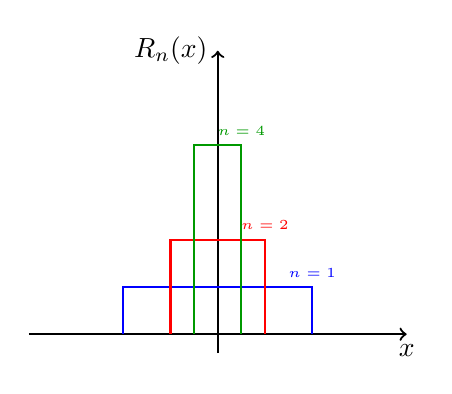
\begin{tikzpicture}[scale=1.2]
                % Axes
                \draw[->, thick] (-2,0) -- (2,0) node[anchor=north] {$x$};
                \draw[->, thick] (0,-0.2) -- (0,3) node[anchor=east] {$R_n(x)$};

                % n=1
                \draw[blue, thick] (-1,0) -- (-1,0.5) -- (1,0.5) -- (1,0);
                \node[blue, anchor=south] at (1,0.5) {\tiny $n=1$};

                % n=2
                \draw[red, thick] (-0.5,0) -- (-0.5,1) -- (0.5,1) -- (0.5,0);
                \node[red, anchor=south] at (0.5,1) {\tiny $n=2$};

                % n=4
                \draw[green!60!black, thick] (-0.25,0) -- (-0.25,2) -- (0.25,2) -- (0.25,0);
                \node[green!60!black, anchor=south] at (0.25,2) {\tiny $n=4$};
            \end{tikzpicture}
            \end{center}
        \end{column}
    \end{columns}
\end{frame}

\begin{frame}{Distributional and Weak Derivatives}
    \textbf{Distributional Derivative}
    \begin{itemize}
        \item For $T \in \mathcal{D}'(\Omega)$ and multi-index $\alpha$, $\partial^\alpha T$ is defined by:
        \[
            \langle \partial^\alpha T, \phi \rangle := (-1)^{|\alpha|} \langle T, \partial^\alpha \phi \rangle \quad \forall \phi \in \mathcal{D}(\Omega) \text{ }.
        \]
        \item If $f \in C^1$, the distributional derivative matches the classical derivative.
    \end{itemize}

    \vspace{0.3cm}
    \begin{block}{Weak derivative}
        If $u \in L^1_{\text{loc}}(\Omega)$ and its distributional derivative $\partial^\alpha T_u$ can be identified with a function $v \in L^1_{\text{loc}}(\Omega)$, then $v$ is the \textbf{weak derivative} of $u$ ($\partial^\alpha u = v$).
    \end{block}
\end{frame}

\begin{frame}{Example: The Heaviside Function}
    Consider the Heaviside function on $\mathbb{R}$:
    \[
        H(x) = 
        \begin{cases} 
            1 & x > 0 \\ 
            0 & x < 0 
        \end{cases} \text{ }
    \]
    
    Calculate the distributional derivative $H'$:
    \begin{align*}
        \langle H', \phi \rangle &= - \langle H, \phi' \rangle \\
        &= - \int_0^\infty \phi'(x) \, dx \text{ } \\
        &= - (\phi(\infty) - \phi(0)) \\
        &= \phi(0) \text{ }
    \end{align*}
    
    Thus, $H' = \delta_0$.
\end{frame}

\section{Sobolev Spaces}

\begin{frame}{Definition of Sobolev Spaces}
    \textbf{The Space $W^{m,p}(\Omega)$}
    \begin{itemize}
        \item For $1 \le p \le \infty$, functions in $L^p(\Omega)$ with weak derivatives up to order $m$ in $L^p(\Omega)$:
        \[
            W^{m,p}(\Omega) := \{ f \in L^p(\Omega) : \forall |\alpha| \le m, D^\alpha f \in L^p(\Omega) \} \text{ }.
        \]
        \item It is a Banach space with the norm:
        \[
            \|x\|_{W^{m,p}(\Omega)} := \sum_{0 \le |\alpha| \le m} \|D^\alpha x\|_{L^p(\Omega)} \text{ }.
        \]
    \end{itemize}
    
    \vspace{0.3cm}
    \textbf{Special Case: $m=1$}
    \[
        W^{1,p}(\Omega) = \{ f \in L^p(\Omega) : \nabla f \in [L^p(\Omega)]^n \} \text{ }.
    \]
\end{frame}

\begin{frame}{Hilbert Sobolev Spaces}
    When $p=2$, the spaces are Hilbert spaces, denoted $H^m(\Omega) = W^{m,2}(\Omega)$.
    
    \vspace{0.3cm}
    \textbf{Inner Product for $H^1(\Omega)$:}
    \[
        (x, y)_{1,\Omega} := (x, y)_{0,\Omega} + (\nabla x, \nabla y)_{0,\Omega} \text{ }.
    \]
    
    \vspace{0.3cm}
    \textbf{Other Fundamental Hilbert Spaces:}
    \begin{itemize}
        \item $H(\text{div}; \Omega) = \{ f \in [L^2(\Omega)]^n : \text{div } f \in L^2(\Omega) \}$.
        \item $H(\text{curl}; \Omega) = \{ f \in [L^2(\Omega)]^3 : \text{curl } f \in [L^2(\Omega)]^3 \}$.
    \end{itemize}
\end{frame}

\begin{frame}{Meyers-Serrin Theorem}
    Alternatively one can define by density
    $$ H^{m,p}(\Omega) = \overline{C^\infty(\Omega)\cap W^{m,p}(\Omega)}^{\|\cdot\|_{W^{m,p}(\Omega)}}$$
    which is easier to manipulate.
    \pause
    \begin{block}{Meyers-Serrin Theorem}
        $$H^{m,p}(\Omega) = W^{m,p}(\Omega) $$
    \end{block}
\end{frame}

\section{Sobolev Embeddings}

\begin{frame}{Example: 1D Embedding into Continuous Functions}
    Consider $I = (a, b)$ and $f \in H^1(I)$. Why does $f \in C^0(I)$?  \pause
    
    By the Fundamental Theorem of Calculus:
    \[
        f(x+h) = f(x) + \int_x^{x+h} f'(s) \, ds \text{ }.
    \]
    Applying Cauchy-Schwarz:
    \begin{align*}
        |f(x+h) - f(x)| &\le \int_x^{x+h} |f'(s)| \, ds \text{ } \\
        &\le \|f'\|_{L^2((x, x+h))} h^{1/2} \text{ } \\
        &\le \|f'\|_{L^2(I)} h^{1/2} \quad \forall x \in I \text{ }.
    \end{align*}
    This shows $f$ is uniformly continuous, directly proving the injection $H^1(I) \hookrightarrow C^0(I)$.
\end{frame}


\begin{frame}{Sobolev Embeddings (Continuous)}
    Let $\Omega \subset \mathbb{R}^d$ be a bounded Lipschitz domain, $m, j \ge 0$ integers, $p \in [1, \infty]$.
    
    \begin{itemize}
        \item \textbf{Case $mp < d$:} For $p \le q \le \alert{\frac{dp}{d-mp}} \text{ (Sobolev critical exponent)} $,
        \[
            W^{j+m,p}(\Omega) \hookrightarrow W^{j,q}(\Omega) \text{ }.
        \]
        \item \textbf{Case $mp = d$:} For $p \le q < \infty$,
        \[
            W^{j+m,p}(\Omega) \hookrightarrow W^{j,q}(\Omega) \text{ }.
        \]
        \item \textbf{Case $mp > d \ge (m-1)p$:}
        \[
            W^{j+m,p}(\Omega) \hookrightarrow C^j(\bar{\Omega}) \text{ }.
        \]
    \end{itemize}
\end{frame}

\begin{frame}{Sobolev Embeddings (Compact)}
    Under similar assumptions ($m \ge 1$, $p \in [1, \infty)$), the following embeddings are \textbf{compact}:
    
    \begin{itemize}
        \item \textbf{Case $mp \le d$:} For $q \in \left[1, \frac{dp}{d-mp}\right)$,
        \[
            W^{j+m,p}(\Omega) \hookrightarrow \hookrightarrow W^{j,q}(\Omega) \text{ }.
        \]
        \item \textbf{Case $mp > d$:}
        \[
            W^{j+m,p}(\Omega) \hookrightarrow \hookrightarrow C^j(\bar{\Omega}) \text{ }.
        \]
    \end{itemize}
    
    \vspace{0.3cm}
    \textit{Crucial Consequence:} $H^1(\Omega)$ is compactly embedded in $L^2(\Omega)$ (Rellich-Kondrachov).
\end{frame}


\begin{frame}
    \maketitle
\end{frame}

\end{document}
